%%================================================
%% Filename: chap03.tex
%% Encoding: UTF-8
%% Author: Yuan Xiaoshuai - yxshuai@gmail.com
%% Created: 2012-04-27 19:47
%% Last modified: 2019-11-07 14:38
%%================================================
\chapter{基于接口号分组标记的溯源防护方法}
% \chapter{基于接口号分组的概率标记法}
\label{cha:IGPPM}
针对传统概率包标记法在进行网络溯源时表现出的溯源准确率不高、溯源速度慢的缺点,本小节对此进行了改进,设计并提出了一种基于路由器接口号分组的概率包标记方案。
与传统依赖于IP地址作为标记信息的方案相比,该方案通过使用路由器接口号作为标记信息,显著减少了对单个路由信息进行标记所需的空间。
此外,通过结合异或运算的特性,本方案能够利用服务器端收集到的数据包标记信息在确保溯源准确率的同时进行快速而准确的路径重构。

% 传统的PPM(概率包标记法)通常使用路由器的IP地址作为标记信息,然而IP地
% 址是相对于全球的网络设备的,占用空间大,为32 bit。故PPM通常只会携带一
% 个路由器的标记信息,这导致了概率包标记法的空间利用率较低,为$1/32 = 
% 0.03125$。这也是为什么传统的概率包标记法需要收集更多数据包以进行路径
% 重构的原因。

% 在本文中,我们将采用一种不同的方案:利用路由器的接口号作为标记信息。IP
% 地址是相对于全球网络设备的,而路由器接口号仅相对于单个路由器内的所有网
% 络接口,所以对单个路由器内的每个接口进行编码将消耗更少的空间。这意味着
% 我们可以在一个数据包中标记多个路由器的信息,提高了标记空间的利用率,从
% 而提高了路径重构的效率,减少了需要收集的数据包数量。这将显著改善数据包
% 标记法进行IP回溯的性能和有效性。

\section{方案总体设计}

本文提出的方案旨在针对网络攻击进行高效、准确地溯源,该方案主要分为三个阶段:路由器标记阶段、标记数据包收集阶段和路径重组阶段。
这三个阶段如图~\ref{fig:our_datapackets_design}~所示。
\begin{figure}[h]
  \centering
  \includegraphics[width = \textwidth]{datapackets.drawio.png}
  \caption{基于接口号分组的概率标记法总体设计}
  \label{fig:our_datapackets_design}
\end{figure}
首先是数据包标记阶段,它是网络追踪的起始步骤,发生在数据包于网络路径上的传输过程中。
当数据包离开发送者设备进入网络后,中间路由器便会根据预设策略对经过的数据包进行概率性标记,写入到本文接下来将要提出的标记信息结构体中,以便路径重构程序有效利用这些信息准确完成路径重构。

其次是标记数据包收集阶段,这一环节主要在受害者服务器上进行。
一旦受害者服务器检测到攻击行为,便会立即启动收集机制,专门对携带标记信息的攻击数据包进行收集。
值得注意的是,这一收集过程与路由器标记阶段可以并行进行,从而提高追踪效率。

当服务器成功收集到足够数量的标记数据包后,便进入路径重组阶段。
在这一阶段,通过利用服务器所收集到的带有标记信息的攻击数据包,执行路径重构算法,我们便能够实现对攻击源的精准定位。
接下来,本文将首先介绍一种专门用于记录数据包标记信息的结构体,随后会围绕前述提到的三个关键阶段展开详细叙述,逐步深入剖析其方案的原理和流程。
\section{标记信息结构体:MarkInfo}
路由器对数据包进行标记的过程,实质上就是路由器将自身的信息写入到数据包的过程。
数据包在网络路径上传输时,可能会经历多个这样的标记过程,直至最终抵达服务器。
对于服务器而言,要完成路径重构,就必须从数据包中提取出这些标记过程产生的信息以及这些信息的关系。
因此,如何在数据包中有效组织并存储这些信息及其关系显得尤为重要。
基于这一需求,本文设计并提出了一种专门在数据包中存储和组织这些标记信息的结构体(如图~\ref{fig:data_structure}~所示):MarkInfo。

\begin{figure}[h]
  \centering
  \includegraphics[width = 0.8\textwidth]{markinfo.drawio.png}
  \caption{本文所设计的用于在数据包中记录标记信息的结构体}
  \label{fig:data_structure}
\end{figure} 

该结构体共由三类字段组成。
首先,是允许标志位(allow\_mark),长度为1 bit。
这一字段的作用是控制后续路由器能否对数据包进行概率标记。
若值为0,则所有路由器均不对该数据包进行标记;若值为1,则后续的组首路由器则会按照预设的概率执行标记操作。
这一设计确保了路径上标记信息的连续性,对于间断式的标记信息,路径重构算法无法有效复原。\par

第二类字段是接口号标记字段(interface\_i),其中i取值范围为[1,m],字段长度为b bit,共可表示$2^b$个接口号。
根据具体的网络环境和溯源需求,b和m的值可灵活调整。

这m个接口号标记字段(interface\_i)在路径重构过程中扮演着核心角色。
每个字段分别记录着数据包在网络传输过程中到达路由器时所经过的输入接口号。
% 具体来说,当数据包在网络中传输时,它会依次经过多个路由器。     
% 在每个路由器上,数据包通过特定的接口进入路由器。
% 这m个接口号标记字段就是用来记录这些接口号的,它们按照数据包经过路由器的顺序进行排列,形成了一组有序的数据。

在本文中,我们将路由器接收到数据包的输入接口号简称为“接口号”,以简化描述并提升表述的清晰度。
\par
% 组的概念是相对于路由器和数据包的,数据包具体要经过的完整路径上的连续m个路由器构成一“组”。


第三类字段则是异或标志位,这类字段共有两个:xor\_1和xor\_2,每个字段与单个接口号标记字段的长度相同。
xor\_1记录的是所有对其标记的路由器的来源接口号异或值;
xor\_2则记录数据包从发送者到接收者整条路径上所有路由器来源接口号的异或值,无论是否进行标记。
这两个字段——xor\_2与xor\_1,在后续的路径重构算法中发挥着不可或缺的作用。
xor\_2结合TTL(生存时间)能够有效区分不同的网络传输路径,而xor\_1则可作为一条关键线索,引导路径重构算法的完成。
具体的重构过程将在后续章节中详细阐述。\par

总的标记空间大小为 $l = 1 + (m + 2) \times b$ bit,用于支持数据包标记过程。
在实际应用中,我们可根据具体场景设定b和m的值。
例如,在本文的实验中,考虑到大多数互联网路由器接口数远少于$2^6 =64$个,我们设定b = 6。
同时,我们设定了 m 分别为 2 和 4,总共使用了 IP 头部中的 25 和 37 bit,对应标记空间的利用率分别为 0.08 和 0.0108。
相较于传统使用 IP 地址作为标记信息的策略(利用率为$1/32 \approx 0.0313$),利用率有了显著提高。
通过这样的结构体,我们能更好的存储数据包在路径传输过程中的收集到的标记信息,方便路径重构算法快速且准确地完成路径重构。\par
% 标记空间具体来自于数据包头部字段,在实际应用时可以依照图2中的IP头部字段来构建此标记空间。
% 在本方案中,我们利用数据包头部中的 b bit来标记数据包经过的路由器来源接口号。
% 每个数据包携带了 m 个接口号标记字段以及两个 XOR (异或)字段,每个 XOR 字段也占据 b bit。
% 最后,还有一个 1 位的允许标志位。总的标记空间大小为 $l = 1 + (m + 2) \times b$ bit,用于支持数据包标记过程。



% 插入外部代码
% \lstinputlisting[firstline=8,style=lstStyleLaTeX]{main.tex}


\section{路由器标记阶段}
\textbf{1. “组”的定义}\par
路由器的数据包标记过程是以“组”为单位进行的。
因此,在本文中,我们将数据包从发送者到接收者所经过的整条路径上每连续的m个路由器划分并定义为一个“组”。
其中,距离发送者最近的“组”被定义为“首组”,而距离接收者最近的“组”则为“最后一组”。
值得注意的是,“最后一组”的路由器数量可能少于m个。
假设从发送者到接收者之间共有d跳路由器,那么这d跳路由器可以被划分为k“组”,其中$k=\lceil d/m \rceil$,即向上取整得到组数。
这样的分组方式有助于我们更有效地进行数据包标记和路径重构。\par

\textbf{2.标记概率的确定}\par
当路由器以组为单位对数据包进行概率标记时,第一组的标记概率为1,即直接进行标记,而其余组则以$p \times allow\_mark$概率进行标记(这里,我们假设p为0到1之间的一个小数)。
另外,需要注意的是,具体的概率判定组是否标记是由组首路由器完成的。
\par

\textbf{3.具体的标记操作}\par
图~\ref{fig:marking_procedure}~是标记操作的详细流程图。
\begin{figure}[h]
  \centering
  \includegraphics[width = 0.8\textwidth]{marking_procedure.png}
  \caption{路由器标记操作流程图}
  \label{fig:marking_procedure}
\end{figure}  
在进行具体的标记操作时,组首路由器会根据先前确定的概率来决定是否对数据包进行标记。\par
若组首路由器决定进行标记,它首先会清空MarkInfo中的所有接口号标记字段(即interface\_i,其中i取值范围为[0,m-1])。
随后,组内的所有路由器将与组首路由器执行相同的操作,检查是否存在空的接口号标记字段。
若存在空字段,则直接将对应的来源接口号填充进去。
同时,计算xor\_1(如公式\ref{eq:xor1}所示)和xor\_2(如公式\ref{eq:xor2}所示)的值,并将它们分别写入相应的异或字段。\par
\begin{equation}
  \label{eq:xor1}
   xor\_1 = xor\_1 \oplus source\_interface
\end{equation}
\begin{equation}
  \label{eq:xor2}
   xor\_2 = xor\_2 \oplus source\_interface
\end{equation}
如果不存在空的接口号标记字段,表明本组均不对此数据包进行标记,接收到该数据包的路由器也将不会对其进行标记。
在这种情况下,路由器仅计算xor\_2的值,并将其写入xor\_2字段中。\par
% xor\_2字段扮演着记录数据包传输路径中所有路由器来源接口号异或值的角色。
% 不论数据包是否在某些路由器处被标记,xor\_2字段都会被更新。
% 这意味着,从发送者到接收者,每经过一个路由器,该路由器都会根据自身的来源接口号计算xor\_2的值,并将这个值写入数据包的xor\_2字段中。
% 这种设计确保了xor\_2字段能够完整反映数据包在网络中的传输路径,为后续的路径重构提供了关键信息。\par

另一方面,如果组首路由器基于概率判断决定不对数据包进行标记,它会将allow\_mark字段的值设置为0。
这一操作是为了通知后续的组,不再对该数据包进行概率性的标记操作。


通过这些操作,当数据包顺利抵达接收者时,其MarkInfo中的interface字段已经记录了一组路由器的接口号。
同时,MarkInfo中的xor\_1字段的值将等于所有对数据包进行标记的路由器接口号的异或,而xor\_2字段的值则等于路径上所有路由器的接口号异或。
当接收者接收到一定数量的标记数据包后便可以提取这些信息执行路径重构算法完成路径重构。
% 在本文的数据包标记法部分,算法~\ref{alg:packet_marking}~提供了详细
% 的内容,用于中间路由器对数据包进行标记,同时,图
% ~\ref*{fig:marking_procedure}~抽象地描述了这一过程。这一过程包括以
% 下关键步骤:

% \begin{algorithm}
    \small
    \caption{Packet Marking Algorithm}
        \begin{algorithmic}[1] %每行显示行号
            
            \Require m

            \Require  packet
            % \Comment{待转发的数据包}

            \Require srcInterface
            % \Comment{数据包在路由器中的来源接口号}

            %if
            \If {packet.TTL == 0}   \State 
                Drop the packet and exit this program
            \Else   
                \State  set INITIAL\_TTL the minimum value greater than Packet.TTL from \{32, 64, 128, 255\}
                \State  index = (INITIAL\_TTL - packet.TTL) \% group\_size
                \If  {index == 0} 
                    \If {packet.TTL == INITIAL\_TTL} \State
                        set all interface  mark fields to empty \State
                        packet.interfaces[0] = srInterface \State
                        packet.xor1 = srInterface \State
                        packet.allowing\_marking = True
                    \ElsIf{packet.allowing\_marking == True}   \State
                        r = random.random()
                        \If{r $<$ marking\_rate} \State
                            set all interface  mark fields to empty \State
                            packet.interfaces[0] = srInterface \State
                            packet.xor1 = packet.xor1 $\oplus$ srInterface \State
                            packet.allowing\_marking = True
                        \Else \State 
                            packet.allowing\_marking = False
                        \EndIf
                    \EndIf
                \ElsIf{packet.interfaces[index] is empty} \State
                    packet.interfaces[index] = srInterface \State
                    packet.xor1 = packet.xor1 $\oplus$ srInterface
                \EndIf  \State
                packet.TTL -= 1 \State
                packet.xor2 = packet.xor2 $\oplus$ srInterface
            \EndIf
            \State
        \end{algorithmic}
        \label{alg:packet_marking}
    \end{algorithm}

% \begin{enumerate}[label=(\alph*).]
%   \item \emph{计算路由器位序:}首先,算法需要确定当前路由器是数据包
%   所经过路径中的第几个路由器,即当前路由器在数据包需要经过的所有路由
%   器的位序。数据包的TTL字段的初始值通常因发送方的系统而异,但通常位于
%   范围{32,64,128,255}内。为实现这一步骤,算法首先读取数据包中的
%   TTL字段,然后从这组初始值中找到能够不小于数据包TTL的值。然后,计算
%   这个最小初始值与数据包中的TTL字段之间的差值,这个差值表示了数据包从
%   发送者发送后到达当前路由器时所经过的路由器跳数,即当前路由器在整个
%   路径中的位序。
%   \item \emph{计算组中序号:}接下来,算法将使用此位序和预定义的组大
%   小参数 m(在伪代码中为\emph{group\_size}变量)进行取模运算,得到
%   模数。本方案利用路由器在数据包从发送者到受害者的整条路径上的顺序,
%   对路由器进行分组。因此,所得的模数表示路由器在组中的序号,范围从0到
%   m-1。
%   \item \emph{区分路由器类型:}根据功能性需求,路由器可以分为两类:
%   组中的0号路由器和非0号路由器。
%   \begin{enumerate}
%     \item[i.] 对于组中的0号路由器,还需要确定是否是路径中首个路由器。
%     如果是首个路由器,便以1概率执行标记操作:将数据包的接口标记字段
%     \emph{interface\_0}到\emph{interface\_(m-1)}全部设置为空,即
%     未标记状态;将数据包在此路由器中的来源接口号写入到相应的接口标记字
%     段;取出XOR1字段中的值与来源接口号进行异或操作,并将结果重新写入到
%     XOR1字段;将数据包中的允许标记字段设置为True。如果路由器非首组的0
%     号路由器,那么它会根据允许标记字段来决定是否以p概率执行标记操作。若
%     标记,操作与前述标记操作相同;若不标记,该路由器会将允许标记字段设置
%     为False。这确保了数据包只有经过本组路由器标记后,后面的其它组才有可
%     能进行标记。
%     \item[ii.] 对于组中非0号路由器,只要数据包中对应的标记字段为空,
%     便会对其进行标记:将来源接口号写入到数据包相应的接口标记字段;取
%     出XOR1字段中的值与来源接口号进行异或操作,并将结果写入到XOR1字段。
%   \end{enumerate}
%   \item \emph{更新数据包信息:}最后的步骤适用于所有中间路由器,无论
%   是否为组中的0号路由器。具体为将来源接口号与XOR2字段值进行异或运算,
%   并将结果重新写入到XOR2字段。这样,XOR2字段结合TTL字段便可作为每条
%   路径的地址。在路径重构过程中,以此即可实现对数据包按路径进行分类。
% \end{enumerate}

% \begin{figure}[htbp]
%   \centering
%   \includegraphics[width = 0.8\textwidth]{marking_procedure.png}
%   \caption{算法~\ref{alg:packet_marking}~流程图}
%   \label{fig:marking_procedure}
% \end{figure} 
\section{标记数据包收集阶段}
\subsection{收集时间}
在正常情况下,当服务器未检测到攻击时,系统不会主动进行标记数据包的收集工作,以确保服务器的正常运行和性能不受影响。
然而,一旦服务器检测到遭受攻击的迹象,便会立即启动标记数据包的收集机制。

\subsection{收集步骤}
标记数据包收集系统的处理步骤如下:

\textbf{1. 初始化路径信息数组}\par
收集系统首先会初始化一个本文设计的如图~\ref{fig:markinfo_list}~所示的路径信息数组(PathInfos),用于管理不同待重构的路径信息。
\begin{figure}[h]
  \centering
  \includegraphics[width = 0.8\textwidth]{mark_list_structure.drawio.png}
  \caption{本文设计的用于管理路径重构信息的数组}
  \label{fig:markinfo_list}
\end{figure} 
该数组包含路径ID(Pid)、路径长度(PLen)以及指向存放标记信息(MarkInfo)数组的指针。
这样的设计使得系统能够高效地存储和检索路径信息。\par

\textbf{2. 提取攻击数据包}\par
系统从网络流量中筛选出与攻击相关的数据包。
这些数据包通常包含特定的攻击特征或标记,以便系统能够准确识别并提取。\par

\textbf{3. 生成路径编码并查找路径}\par
收集系统将攻击数据包中的TTL字段和MarkInfo中的xor\_2字段拼接生成路径编码。
TTL字段指示数据包在网络中的生存时间,而xor\_2字段记录数据包经过的所有路由器来源接口号的异或值。
利用这两个字段的组合,系统能够为每条传输路径生成唯一的编码。
随后,系统利用这个路径编码在PathInfos中查找是否存在相应的路径信息。
如果找到匹配项,则进入步骤5;否则,进入步骤4。\par

\textbf{4. 初始化新路径信息}\par
当PathInfos中不存在与当前路径编码匹配的信息时,系统执行以下操作:
\begin{enumerate}[label=\roman*.]
  \item 计算路径长度;
  \item 将路径长度和路径编码添加到PathInfos中相应元素的字段中;
  \item 分配内存空间用于存放新路径的标记信息数组,并更新PathInfos中对应元素的指针,使其指向该数组;
  \item 启动一个针对新路径的重组程序,并建立与该路径的发布者订阅者关系。
\end{enumerate}
\par

\textbf{5. 写入标记信息并通知重组程序}\par
执行完步骤4后,PathInfos中已经存在与当前路径编码匹配的信息,此时执行以下操作:
\begin{enumerate}[label=\roman*.]
  \item 从当前操作的攻击数据包中提取MarkInfo;
  \item 将提取的MarkInfo追加到对应路径的标记信息数组中;
  \item 通知在该路径上进行订阅的重组程序进行处理。
\end{enumerate}
\par
\textbf{6. 重复执行直至停止溯源}\par
从第2步到第5步的操作将重复执行,直到系统接收到停止溯源的指令或网络流量中不再出现与攻击相关的数据包为止。\par

通过这些操作的循环执行,收集系统能够实现对网络流量的持续监控,确保及时捕获与攻击相关的数据包。
同时,系统也能够及时通知路径重构程序进行实时溯源,从而高效处理海量网络数据。
% \subsection{收集步骤}
% 标记数据包收集系统的工作流程如下:\par
% \textbf{1.初始化路径信息数组:PathInfos}
% 收集系统首先会初始化如图~\ref{fig:markinfo_list}~所示的数组(PathInfoList)对不同待重构的路径进行管理。
% \begin{figure}[h]
%   \centering
%   \includegraphics[width = 0.8\textwidth]{mark_list_structure.drawio.png}
%   \caption{本文设计的用于管理路径重构信息的数组}
%   \label{fig:markinfo_list}
% \end{figure} 
% 数组中共有三个字段,第一个字段(Pid)是路径的ID,即路径的唯一标志值,第二个字段(PLen)是该路径的长度,第三个字段是一个结构体数组的指针,该指向存放MarkInfo的数组。


% \textbf{2.攻击数据包提取:}
% 初始化完PathInfoList后系统首先会从网络流量中筛选出一个与攻击相关的数据包。
% 这种数据包通常包含特定的攻击特征或标记,以便系统能够准确识别并提取。\par


% \textbf{3.路径查找:}
% 收集系统将攻击数据包中的TTL(Time-To-Live)字段值以及MarkInfo中的xor\_2字段的值进行拼接。
% xor\_2字段记录了数据包经过的所有路由器来源接口号的异或值,而TTL字段则指示了数据包在网络中的生存时间。
% 通过这两个字段的组合,系统能够为每条传输路径生成一个独特的编码作为路径编码。\par
% 然后收集系统利用这个路径编码去PathInfoList种查找,看看数组中是否已经存在这样的路径信息。
% 如果存在转到转到步骤5,如果不存在,转到步骤4。

% \textbf{4.初始化标记信息数组:}
% 收集系统首先会计算路径长度。
% 并将路径长度和路径编码分别追加到数组中的元素内。
% 之后收集系统开辟一个存放标记信息的数组,并使元素的指针指向该数组。
% 最后系统会开启一个专门针对此路径进行重组的程序,该程序和此路径建立发布者订阅者关系。\par

% \textbf{5.标记信息写入:}
% 收集系统将当前操作的攻击数据包中的MarkInfo提取并追加到相应的标记信息数组中。
% 并通知在该路径上进行订阅的路径重组程序进行处理。\par
% \subsection{收集时间}
% 在正常情况下,当服务器未检测到遭受攻击时,系统不会主动进行标记数据包的收集工作,以确保服务器的正常运行和性能不受影响。
% 然而,一旦服务器检测到遭受攻击的迹象,便会立即启动标记数据包的收集机制。

% \subsection{收集步骤}
% 标记数据包收集系统首先会将所有的攻击数据包提取。
% 之后将这些数据包依据标记MarkInfo中的xor\_2字段以及TTL字段进行拼接以此作为每条路径的编码。
% 收集系统并维持许多队列,每个队列对应一条路径,其中存储着所有走过该路径的攻击数据包。
% 因此每当收集系统接收到一个攻击数据包时便会将其放入路径对应的队列中,并通知在该队列上进行路径重组的线程进行路径重构。
\section{路径重组阶段}
一旦PathInfos中出现相应的路径信息,路径重组程序便被创建。
路径重组程序的流程如下:\par
\textbf{1.初始化变量:}\par
\begin{enumerate}[label=\roman*.]
  \item 创建一个cur\_xor变量,初始值设为xor\_2(注意:此时该数组中所有的MarkInfo的xor\_2值均相同)。该变量将作为路径重构的关键线索。
  \item 创建一个cur\_len变量,初始值设为0。用于记录当前路径重构的长度。
  \item 初始化一个路径重构队列path\_queue,用于存储重构过程中得到的接口号序列。
\end{enumerate}

\textbf{2.查找匹配的MarkInfo:}
\begin{enumerate}[label=\roman*.]
  \item 从对应的MarkInfo数组中查找是否存在MarkInfo.xor\_1与cur\_xor相等的记录。
  \item 如果找到匹配项,进入步骤4;否则,进入步骤3。
\end{enumerate}

\textbf{3.等待新数据:}
\begin{enumerate}[label=\roman*.]
  \item 将当前重组程序置为阻塞状态,等待收集系统发布新的MarkInfo数据。
  \item 当接收到新数据时,判断其MarkInfo.xor\_1是否与cur\_xor相等。
  \item 如果相等,进入步骤4;否则,继续阻塞并等待新数据。
\end{enumerate}

\textbf{4.更新路径重构信息:}
\begin{enumerate}[label=\roman*.]
  \item 将找到的MarkInfo中的interface\_i逆序放入path\_queue中。
  \item 根据公式重新计算cur\_xor的值,计算方式如公式~\ref{eq:calculateXor}~所示。
\begin{equation}
  \label{eq:calculateXor}
  cur\_xor = cur\_xor \oplus interface\_1 \oplus interface\_2 \oplus \cdots \oplus interface\_m
\end{equation}
  \item 更新cur\_len的值:cur\_len = cur\_len + m。
\end{enumerate}

\textbf{5.判断路径重构状态:}
\begin{enumerate}[label=\roman*.]
  \item 比较cur\_len与PLen的值。
  \item 如果cur\_len等于PLen,进一步检查cur\_xor是否等于0。
  \item 如果cur\_xor不等于0,表明构建失败,进入步骤6。
  \item 如果cur\_xor等于0,表明构建成功,进入步骤7。
  \item 如果cur\_len不等于PLen,表明路径重构尚未完成,返回步骤2并按照当前的路径重构状态继续匹配MarkInfo完成重构。
\end{enumerate}


\textbf{6.处理构建失败情况:}\par
如果路径构建失败,可能是由于数据不完整或路径信息错误。
此时,可以根据实际情况选择重新收集数据或标记该路径为无效。\par

\textbf{7.返回重构结果:}\par
如果路径构建成功,返回path\_queue中存储的接口号序列作为重构结果。
% 1.创建cur\_xor变量,并设初值为xor\_2(注意:此时该数组中所有的MarkInfo.xor\_2均相同)。此变量用以作为路径重构的线索。
% 创建cur\_len变量,并设初值为0,此变量表示当前路径重构的长度。
% 创建路径重构队列path\_queue中,用以存放重构的接口号。\par
% 2.从对应的MarkInfo数组中查找是否存在MarkInfo.xor\_1与cur\_xor相等。
% 如果不存在转到步骤3,如果存在转到步骤4。\par
% 3.当前重组程序进入阻塞状态,等待收集系统发布新的消息。
% 倘若有消息出现重组程序进入唤醒状态并判断新加入的数据包MarkInfo.xor\_1是否与cur\_xor相等。
% 若相等转到步骤4。否则继续阻塞等待新消息。\par
% 4.将MarkInfo中所有的MarkInfo.interface\_i逆序放入到path\_queue中,并重新计算cur\_xor的值。计算方式如公式所示。
% \begin{equation}
%   \label{eq:calculateXor}
%   cur\_xor = cur\_xor \oplus MarkInfo.interface\_1 \oplus MarkInfo.interface\_2 \oplus \cdots \oplus MarkInfo.interface\_m
% \end{equation}
% 计算cur\_len的值:cur\_len = cur\_len + m。\par
% 5.判断cur\_len的值是否已经等于PLen:如果相等继续判断cur\_xor是否等于0,如果不等于0,表明构建失败转到步骤6;如果等于0则表明构建成功,转步骤7;
% 如果cur\_xor不等于PLen,表明构建尚未完成转到步骤2。\par
% 7.构建成功,返回path\_queue中存储的接口号序列。\par
% \section{路径重组阶段}
% 一旦受害者服务器在检测到攻击后,便会开始收集攻击数据包。当收集到的数
% 据包数量达到一定阈值时,受害者服务器就会进入收敛状态。在这个状态下,服
% 务器会利用其中带有标记的攻击数据包来进行路径重构。算法~\ref{alg:path_reconstruction}~提供了受害者服务器如何在这个过程中
% 利用标记数据包进行路径重构的详细内容。路径重构的流程为:

% \begin{algorithm}[htbp]
    \small
    \caption{Path Reconstruction Algorithm}
    \begin{algorithmic}[1] %每行显示行号

        \Require $S$ \Comment{all marked packets set recived in victim}
        \Ensure $result\_router\_paths$
        \State Initial an empty set $S'$
        \State Initial an empty set $result\_interface\_paths$
        \State Initial an empty set $result\_router\_paths$
        \State is\_multiple\_of\_group\_size = (INITIAL\_TTL - key\_TTL)\%group\_size == 0
        \Comment{Indicate whether the path length is a multiple of the group length}
        \State partition $S$ into different subsets and add in set $S'$ based on packet.TTL and packet.xor2 fields 
        %if
        \For{each subset $U$ in set $S'$} 
            \State Initial an empty set $T$ \Comment{The root data packets used for reconstruction}
            \State  set INITIAL\_TTL the minimum value greater than Packet.TTL from \{32, 64, 128, 255\}
            \For{each packet in subset $U$}
                \State set interface\_count to count of valid interfaces in packet's mark field
                \If{is\_multiple\_of\_group\_size }
                    \If{interface\_count $\not=$ group\_size}
                        \State $U$ = $U$-\{packet\}
                    \ElsIf {packet.xor1==packet.xor2}
                        \State  $T$ = $T$+\{packet\}
                    \EndIf
                \ElsIf {interface\_count $\not=$ group\_size}
                    \State $U$ = $U$-\{packet\}
                    \If {interface\_count == (INITIAL\_TTL - key\_TTL) \% group\_size and packet.xor1 == packet.xor2}
                        \State $T$ = $T$+\{packet\}
                    \EndIf
                \EndIf
            \EndFor
        
            \For {each packet in set $T$}
                \State Initial an empty set $current\_interface\_path$
                \State remaining\_ipath\_length = INITIAL\_TTL - key\_TTL
                \State flag = \Call{try\_construct}{packet, $U$,$result\_interface\_paths$, $current\_interface\_path$,remaining\_ipath\_length}   
                \If{flag == False and is\_multiple\_of\_group\_size}
                    \State $U$ = $U$+\{packet\} \Comment{Restore $U$ to its state before calling 'try\_construct'}
                \EndIf
            \EndFor
        \EndFor
        

        \For{each $interface\_path$ in $result\_interface\_paths$}
            \State current\_router = victim\_router
            \State $reconstructed\_path$ = \{current\_router\}
            \For{each interface\_num in $interface\_path$}
                \If {interface\_num - 1 $<$ len(neighbors,current\_router)}
                    \State next\_router = get\_router\_by\_interface(interface\_num,current\_router)
                    \State $reconstructed\_path$ = $reconstructed\_path$ + \{next\_router\}
                    \State current\_router = next\_router
                \Else
                    \State $reconstructed\_path$ = \{\}
                    \State break
                \EndIf
            \EndFor

            \If {len($reconstructed\_path$) $>$ 0}
                \State $result\_router\_paths$ = $result\_router\_paths$+ reverse($reconstructed\_path$)
            \EndIf

        \EndFor
    \end{algorithmic}
    \label{alg:path_reconstruction}
\end{algorithm}

% \begin{enumerate}[label=(\alph*).]
%   \item \emph{划分攻击数据包结合S:}首先,将攻击数据包集合 $S$ 根据
%   数据包的 XOR2 字段和 TTL 字段的不同值划分为不同的子集 $U_i$ ,并
%   将这些子集全部添加到集合 $S'$ 中。
%   \item \emph{根数据包集合的收集与干扰数据包排除:}接下来,对 $S'$ 
%   中的每个子集$U_i$进行遍历,从每个子集$U_i$中收集根数据包并添加到根
%   数据包集合 $T$ 中,并将这些根数据包以及可能的干扰数据包从子集 
%   $S_i'$ 中剔除。
%   \item \emph{获取接口号路径:}针对步骤(b)所得到的根数据包集合 
%   $T$,利用这些根数据包以及相应的子集$U_i$,调用算法
%   ~\ref*{alg:try_construct}~进行路径重构,从而得到路由器接口号的路
%   径。
%   \item \emph{获取攻击路径:}利用步骤(c)所得到接口号路径逐个查询路
%   由器最终获得路径上的所有路由器。
% \end{enumerate}

% 步骤(a),由于来自同一结点且走过相同路径的数据包的 TTL 值必定相同,同
% 时数据包中的 XOR2 字段包含了从攻击者到受害者服务器的整条路径上的所有
% 路由器的接口号的异或值,因此,首先结合数据包中的 XOR2 字段和 TTL 字
% 段将攻击数据包集合分成不同的子集。

% 对于步骤 (b) 和步骤 (c) ,由于在我们的算法中,XOR1字段只会在路由器进
% 行标记时才重新计算并写入,如果不进行标记,那么 XOR1字段将与路由器接口
% 字段保持不变。改变的只有 XOR2 字段,因为 XOR2字段反映了整个数据包所
% 经过的路径,而 XOR1 字段只记录了已标记的路由器。我们的方案具有这样的
% 特性,假设攻击数据包在经过$ R_1 \dots R_i \dots R_d $ 后到达受害者
% ($ i \in [1,d] $表示距离发送者的路由器跳数),$ \{R_{x_1} \dots 
% R_{x_n}\}$($n \in [2,d]$)依次对其进行了标记,对应$ XOR1 = R_{x_1}
%  \oplus \dots \oplus R_{x_n}$,那么有$x_j - x_{j-1} = 1,j \in 
%  [2,n]$。因此,我们可以使用 XOR1 字段作为线索来按序获取整条路径上的
%  所有路由器接口号,这些按顺序排列的路由器接口号序列即可表示它们所走过
%  的完整路径,我们将这些由有序的路由器接口号序列所表示的路径称为接口号
%  路径。获取接口号路径的具体方法是首先找到 XOR1=XOR2 的数据包,这些数
%  据包记录了到达受害者的最后一跳路由器接口号,可以看作线索的头部。在本
%  文中,我们将这些数据包称为根数据包。因此,步骤 (b) 的任务是从每个子
%  集中提取出根数据包集合T,并在步骤 (c) 中使用算法
%  ~\ref*{alg:try_construct}~来获取路由器接口号路径。

% 步骤(d),将利用这些接口号路径来获取实际的攻击路径。具体方法是,受害者
% 服务器首先从自己的网关路由器开始,递归查询路由器接口号对应的上游路由
% 器,直到查询完所有路由器接口号对应的路由器结点,从而获得路由器结点路
% 径,也就是攻击路径。

% \section{Try Construct Procedure算法}

% 接下来我们将会详细介绍算法~\ref*{alg:try_construct}~的内容。



% \begin{enumerate}[label=(\alph*).]
%   \item 将base\_packet中的所有接口号逆序添加到当前尝试构建的接口路
  
%   径current\_interface\_path中,
%         并重新计算算法中的xor1变量、添加的接口号个数append\_num、该路径剩余的接口号个数remaining\_ipath\_legth。
%   \item 若remaining\_ipath\_legth = 0,执行步骤(c),否则执行步骤(f)。
%   \item 若xor1此时为空值执行步骤(d),否则执行步骤(e)。
%   \item 将当前尝试构建的接口号路径current\_interface\_path添加到接口号路径结果集合result\_interface\_path中,再将current\_interface\_path置为空后返回构建结果True。
%   \item 从当前尝试构建的接口号路径current\_interface\_path中去掉刚添加的append\_num个接口号,返回构建结果False。
%   \item 遍历集合U,从U中根据xor1变量的值收集下一个所有可能的标记数据包base\_packet,并将它们添加到集合packets中。遍历完U后,若集合packets的长度为0执行步骤(g),否则执行步骤(h)。
%   \item 从当前尝试构建的接口号路径current\_interface\_path中去掉刚添加的append\_num个接口号,返回构建结果False。
%   \item 遍历packets集合中的每个packet,从集合U中去掉packet,将packet作为新的base\_packet递归调用本过程开始下一轮尝试构建,并取得尝试构建的结果。若构建成功,向上层调用返回结果True,否则再将本次递归调用使用的packet添加到U中,继续遍历,直到遍历完packets集合中所有的packet。
%   \item 从当前尝试构建的接口路径current\_interface\_path中去掉刚添加的append\_num个接口号,向上层调用返回构建结果False。
% \end{enumerate}


% 在算法~\ref*{alg:try_construct}~中我们使用xor1变量作为依次找到包含相关路由信息的数据包线索。而变量append\_num则用于记录每次构建过程中向current\_interface\_path添加的接口号数量,这在构建失败时可以用来恢复current\_interface\_path到之前的状态。remaining\_ipath\_length 控制了current\_interface\_path的长度,当remaining\_ipath\_length为0时,将不能再向current\_interface\_path添加接口号。此时有两种可能结果:构建成功或构建失败。如果xor1为0,可能构建成功;否则必定失败。如果remaining\_ipath\_length不为0,表示路径仍未完整,需要继续利用xor1作为线索,逐一尝试构建数据包,直到构建成功或失败,下面是算法3.3的相关伪代码。

% \begin{algorithm}[htbp]
    \small
    \caption{TRY\_CONSTRUCT Procedure}
    \begin{algorithmic}[1] %每行显示行号
        \Procedure{try\_construt}{base\_packet,$U$,$current\_interface\_path$, 
        $result\_interface\_paths$,remaining\_ipath\_length}
        \State xor1 = base\_packet.xor1 
        \State $packet\_path$ = reverse(base\_packet.interfaces\_group) \Comment{Reverse sequence of interface numbers in the data packet}
        \State append\_num = 0
        \For {each interface\_num in $packet\_path$}
            \If{interface\_num $\not=$ EMPTY\_VALUE}
            \State  $current\_interface\_path$ = $current\_interface\_path$ + \{interface\_num\}
            \State append\_num += 1
            \State remaining\_ipath\_length -= 1
            \State xor1 = xor1 $\oplus$ interface\_num
            \EndIf
        \EndFor
        \If{remaining\_ipath\_length == 0}
            \If{xor1 == EMPTY\_VALUE}
                \State $result\_interface\_paths$ +=  $current\_interface\_path$
                \State $current\_interface\_path$ = \{\}
                \State \Return True
            \Else
                \State remove the last append\_num items from $current\_interface\_path$
                \State \Return False
            \EndIf
        \Else 
            \State Initial an empty set $packets$
            \For {each packet in $U$}
                \If {packet.xor1 == xor1}
                    \State $packets$ += \{packet\}
                \EndIf
            \EndFor
            \If {$|packets|$== 0}
                \State remove the last append\_num items from $current\_interface\_path$
                \State \Return False
            \Else
                \For{each packet in $packets$}
                    \State $U$ = $U$ - \{packet\}
                    \State flag = \Call{try\_construct}{packet, $U$,$result\_interface\_paths$,
                    $current\_interface\_path$,remaining\_ipath\_length} 
                    \If{flag == True}
                    \State \Return True
                    \Else
                        \State $U$ += \{packet\}
                    \EndIf
                \EndFor
                \State remove the last append\_num items from $current\_interface\_path$
                \State \Return False
            \EndIf
        \EndIf
        \EndProcedure 
    \end{algorithmic}
    \label{alg:try_construct}
\end{algorithm}

% 为了更容易理解这一过程,图~\ref*{fig:try_construct}~表示了算法~\ref*{alg:try_construct}~的流程图。
% \begin{figure}[htbp]
%   \centering
%   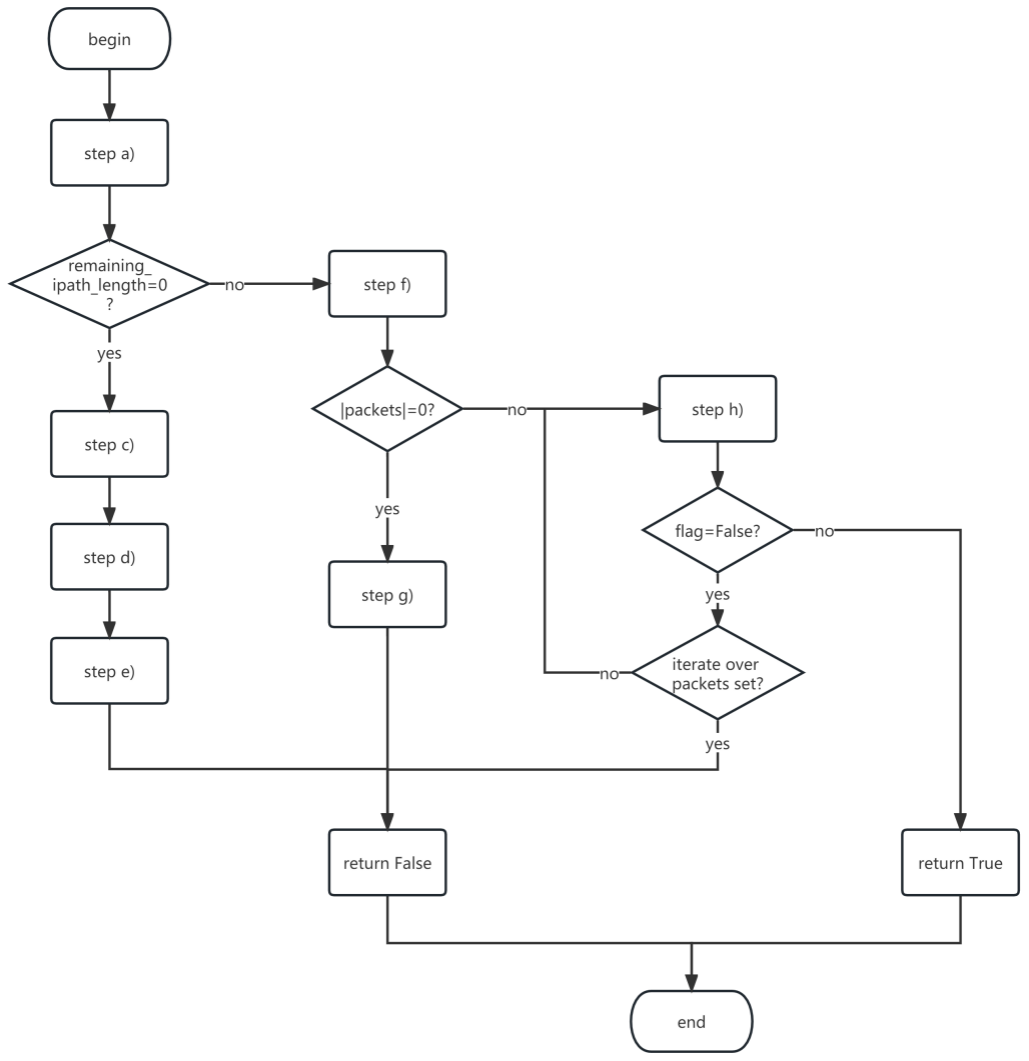
\includegraphics[width = 0.8\textwidth]{try_construct.png}
%   \caption{算法~\ref*{alg:try_construct}~流程图}
%   \label{fig:try_construct}
% \end{figure} 

% \section{概率模型和最小期望的数据包数}
% \label{sec:mainbody} 
% 假设攻击者距离受害者服务器有d跳,IGPPM方案中数据包记录m个路由器接口
% 号,则从攻击者到受害者服务器的完整路径中的所有路由器总共可分为$k = 
% \lceil d/m \rceil$组,标记概率为p。不同于传统概率包标记法的概率模型
% ,本方案只有当前一组路由器进行标记后,后一组路由器才可进行p概率确定
% 是否标记;若前一个路由器不标记,那么之后的所有路由器也将不会进行标
% 记,这将导致则受害者服务器在收到一个标记数据包时,此标记数据包携带
% 第i组路由信息的概率为:
% \begin{equation}
%   \label{eq:Probability of i-th Router}
%   f(i) = 
%   \begin{cases} 
%     p^{i-1}(1-p), & 1 \leq i \leq k-1 \\
%     p^{k-1}, & i = k 
%   \end{cases}
% \end{equation}
% 因此受害者服务器收集的数据包数量能够覆盖所有路由器是由
% \begin{equation}
%   \label{eq:Path Coverage Probability}
%   g(p) = \min\{(1 - p), p(1 - p), \ldots, p^{k-2}(1 - p), p^{k-1}\}
% \end{equation}
% 所决定的,完成路径重构所需的最少数据包数量为:
% \begin{equation}
%   \label{eq:Minimum Packets for Path Reconstruction}
%   z(p) = \frac{1}{g(p)} = \frac{1}{\min\{(1 - p), p(1 - p), \ldots, p^{k-2}(1 - p), p^{k-1}\}}
% \end{equation}


% 要使$z(p)$取最小值,只需$g(p) = \min\{(1 - p), p(1 - p), \ldots, p^{k-2}(1 - p), p^{k-1}\}
% $取最大值即可。其中$\min\{(1 - p), p(1 - p), \ldots, p^{k-2}(1 - p)\} = p^{k-2}(1 - p)$,因此$g(p) = \min\{(1 - p), p(1 - p), \ldots, p^{k-2}(1 - p), p^{k-1}\}
%  = \min\{p^{k-2}(1 - p), p^{k-1}\}$。进一步分析知,当$p<1/2$时,$p^{k-1}<p^{k-2}(1 - p)$,此时$g(p) = p^{k-1}$;当$p>1/2$时,$p^{k-2}(1 - p)<p^{k-1}$,此时$g(p) = p^{k-2}(1 - p)$
% ,即
% \begin{equation}
%   \label{eq:Simplified Probability of i-th Router}
%   g(p) = 
%   \begin{cases} 
%     p^{k-1}, & p \leq \frac{1}{2} \\
%     p^{k-2}(1 - p), & p > \frac{1}{2}
%   \end{cases}
% \end{equation}

% 再进一步分析知当$k>2$时,$p = \frac{k-2}{k-1}$,$g(p)$最大;当$k \leq 2$,
% $p = 1/2$时,$g(p)$最大。也就是说当$k = \lceil d/m \rceil >2$时,
% $p = \frac{k-2}{k-1}$,完成路径重构所需数据包数量最少,为
% $\frac{(k-1)^{k-1}}{(k-2)^{k-2}}$,当$k = \lceil d/m 
% \rceil \leq 2$,$p = 1/2$,完成路径重构所需数据包数量最少为
% $2^{k-1}$。

\section{实验设计和结果分析}
\label{sec:bib}
为了验证本方案进行路由回溯的速度与准确性,本文设置了两组对比实验分别验证这两个指标。
首先,在第一组实验中,我们利用CAIDA IPv4 Prefix-Probing Traceroute数据集构建了网络拓扑,并选定受害者结点。
随后,从距离受害者不同距离的结点处向受害者结点发送数据包,以测试完成路径重构所需要收集的数据包数量,从而反映回溯速度。
我们将这一结果与PPM-Dynamic和PPM-Fixed方案进行了细致地对比,以全面评估本方案的性能。\par

接着,第二组实验则侧重于准确性的验证。
我们利用NS-3模拟器创建了一个网络仿真环境,并在此环境中利用网络结点向服务器发送大量数据包模拟DDos攻击。
通过这一实验,我们能够准确地评估本方案在进行路径重构时的准确率,从而确保其在实际应用中的可靠性。
以下是对这两组实验的详细解读与结果分析。

\subsection{溯源速度测试}
\textbf{1.数据集介绍}\par
CAIDA IPv4 Prefix-Probing Traceroute Dataset由CAIDA提供,包含20,377,233条路径追踪记录。
这些记录涵盖了899,916个不同的IP地址。注意,本文只使用了可以到达指定目的地且没有循环的部分路径追踪记录。\par
% 数据集中的接口级(Interface level)跳数长度最小为1,最大为31,平均跳数长度为15.43。\par
\textbf{2.实验评估指标}\par
在本次溯源速度测试中,我们使用完成路径重构所需收集的数据包数量作为关键验证指标。
数据包数量是衡量溯源速度的重要指标之一,因为它直接关系到网络路径回溯或安全分析任务的执行效率和速度。
通过减少完成溯源所需的数据包数量,可以显著提升溯源的速度,从而更快地获取分析结果。
这不仅能够减少网络负载,降低资源消耗,还能提高整体分析效率,为网络安全的实时监测和响应提供有力支持。
因此,在本次实验中,我们重点验证了本方案在减少数据包数量方面的优势。\par

\textbf{3.实验设计}\par
本文从数据集中筛选出跳数达到最大的追踪记录,并将这些记录中的目的结点作为受害者结点。
随后,我们按照距离d从1开始递增的方式,随机选取距离受害者d跳的结点,模拟攻击结点向向受害者结点发送攻击数据包。
受害者结点负责收集这些数据包,并应用路径重构算法来还原数据包的传输路径。
为了确保实验结果的可靠性和一致性,我们对每个距离d都进行了1,000次重复实验并取平均值。
此外,为了模拟更真实的实验环境,我们还引入了一些额外的结点作为用户结点。
这些用户结点模拟了实际网络中的其他用户活动,增加了实验的复杂性和真实性。\par
\textbf{4.实验结果与分析}
% 图~\ref*{fig:packets_num}~显示了本方案在 $m=2$ 和 $m=4$ 的情况下,与 PPM-Fixed 
% 和 PPM-Dynamic 方案相比,完成不同距离的路由回溯,达到95\%成功率所需的最少数据包数
% 量与路径长度之间的关系。

% 可以看出,本文提出的方案在完成路径重构时所需要的数据包数量要远远少于PPM-Fixed方案。
% 当m=2时本方案略优于PPM-Dynamic方案,当m=4时则明显优于以上两种PPM类方案。另外,
% 仔细观察图像可以发现,本文提出的方案表现出阶梯性特征,这是因为该方案采用了分组
% 标记的方法:不管跳数d相差多少,只要$k = \lceil d/m \rceil$相同,完成路径重构所需
% 要的数据包数量就会相同。

图\ref{fig:packets_num}是本方案在m=2和m=4的情况下,与PPM-Fixed和PPM-Dynamic方案相比,完成不同距离的路由回溯所需的最少数据包数量与路径长度之间的关系。
\begin{figure}[htbp]
  \centering
  \includegraphics[width = 0.8\textwidth]{packets_num.png}
  \caption{路径重建所需数据包数量与路径长度关系}
  \label{fig:packets_num}
\end{figure} 
从图中可以看出,本文提出的方案在完成路径重构时所需要的数据包数量要远远少于PPM-Fixed方案。
当m=2时,本方案略优于PPM-Dynamic方案;当m=4时,则明显优于以上两种PPM类方案。
这一结果表明,本方案在溯源速度方面具有显著优势。
此外,仔细观察图像可以发现,本文提出的方案表现出阶梯性特征。
这是因为该方案采用了分组标记的策略:无论跳数d相差多少,只要$k=\lceil d/m \rceil$相同,完成路径重构所需要的数据包数量就会相同。
通过以上的实验验证和结果分析,本方案相较于传统的PPM方案,在溯源速度方面展现出了明显的优越性。\par

另外值得注意的是,在传统的PPM类方案中,路径重构所需的数据包数量通常指的是实现路由覆盖所需的最少数据包数量。
因此,在本文中,对于PPM完成路径重构所需的数据包数量的评估,实际上仅是基于路径覆盖测试的数据包统计。
实际上,如果期望通过数据包的数量关系直接获取一条完整的网络路径,那么所需的数据包数量将会非常庞大。
不过,本文所提方案在完成路径重构时,采用了接口号以及两个异或字段以及TTL来实现溯源,这使得本文的方法在路径重构时具有更高的灵活性和效率。
因此,在本文的方案中,完成路径重构所需的数据包数量即为取得一条实际路径所需的数据包数量,这大大减少了重构路径所需的数据包开销。
\subsection{溯源准确率测试}
\textbf{1.仿真软件介绍}\par
在本次实验中本文使用NS-3网络模拟器来构建实验环境。
NS-3是一个先进的开源网络模拟器,广泛应用于网络研究和教育领域,它通过离散事件模拟技术支持各种有线、无线网络协议和设备的性能评估。
该模拟器以其模块化设计和丰富的模型库而闻名,允许用户灵活构建复杂的网络场景。\par
% NS-3的主要开发语言是C++,但它也提供了Python绑定,增加了编程的灵活性和易用性。
% 它被设计来模拟实际网络环境中的行为,帮助研究人员在受控的环境下测试和验证网络算法和协议的性能。
% 得益于其广泛的文档、示例代码和一个活跃的开源社区,NS-3对于那些希望深入理解网络原理、设计新的网络协议或评估网络安全机制的人来说,是一个极为宝贵的资源。
\textbf{2.实验设计}\par
本文首先借助NS-3仿真工具构建了一个如图~\ref{fig:network_enviroment}~所示的逻辑拓扑网络,其中包含14个转发结点($R_i$,其中i的范围是1到14),10个作为攻击者结点的数据发送结点($PC_j$,其中j的范围是1到10),以及一个作为受害者结点的数据接收结点(Server)。
\begin{figure}[h]
  \centering
  \includegraphics[width=0.8\textwidth]{network_enviroment.drawio.png}
  \caption{NS-3模拟器生成的逻辑拓扑结构}
  \label{fig:network_enviroment}
\end{figure}
为了评估网络在不同攻击规模下的性能表现,我们首先使用5个攻击结点向受害者结点发送攻击数据包。
随后,我们逐步增加攻击结点的数量,以模拟网络遭受更大规模攻击的场景。
当攻击结点数量超过10个时,我们采取了以$R_5$为网络拓扑中心随机添加转发结点的策略,并在每个新添加的转发结点上挂载一个攻击结点,以模拟攻击行为的进一步扩散和复杂化。
以下是本次实验的结果与分析部分。\par
\textbf{3.实验结果与分析}\par
图~\ref{fig:traceback_accuracy}~是我们的方案与ICMP Ping方案以及PPM方案在网络仿真环境下的对比结果。
\begin{figure}[h]
  \centering
  \includegraphics[width=0.8\textwidth]{traceback_accuracy.png}
  \caption{拓扑还原准确率}
  \label{fig:traceback_accuracy}
\end{figure}

从图中可以看出,随着攻击结点数的不断增加,本文的所提出的方案准确率相对较高并且相对稳定。
而ICMP Ping方案以及PPM方案随着结点数的增加,溯源准确率极速下降。
因此我们可以得出结论,对于较大规模的网络攻击,本文的所提出的方案仍能以较高的准确率完成溯源任务。
\section{本章小结}
% 在本章中,我们提出了一种基于路由器接口号分组的概率包标记溯源方案。
% 随后我们对本方案的设计从设计的记录标记信息的结构体、路由器的标记阶段的原理和流程、标记数据包收集的原理和流程、路径重构阶段的流程逐步展开叙述。
% 最后我们进行了一系列的实验评估,分别测试了本文所提方案在溯源速度以及准确率方面的表现,经实验结果显示我们的方案在溯源速度和准确率方面均表现优异。
在本章中,本文提出了一种基于路由器接口号分组的概率包标记溯源方案。
首先,本文介绍了该方案的设计架构和设计目的:旨在提高传统概率包标记溯源方案的溯源速度和准确性。
接着,本文深入阐述了方案的设计细节,包括记录标记信息的结构体设计、路由器标记阶段原理和流程、标记数据包收集的原理和流程以及路径重构阶段的流程。
最后,为了验证本方案的性能,本文进行了一系列实验评估,分别测试了本方案在溯源速度以及准确率方面的表现,经实验结果表明,本文的所提出的方案在溯源速度和准确率方面均表现出色。
% 为了验证本文所提方案的路由回溯能力,我们设计了在单个攻击者环境下的路由回溯实验。
% 图~\ref*{fig:packets_num}~显示了本方案在 $m=2$ 和 $m=4$ 的情况下,与 PPM-Fixed 
% 和 PPM-Dynamic 方案相比,完成不同距离的路由回溯,达到95\%成功率所需的最少数据包数
% 量与路径长度之间的关系。其中IGPPM方案与PPM-Fixed方案所采用的标记概率分别为
% $p_{IGPPM}=\frac{k-2}{k-1}$,$p_{PPM-Fixed} = \frac{1}{d}$,也即$p$的选择能够分
% 别使这几种回溯方案的回溯能力达到最佳状态,完成IP回溯所需要的数据包数量最少。

 
% 可以看出,本文提出的方案在完成路径重构时所需要的数据包数量要远远少于PPM-Fixed方案。
% 当m=2时本方案略优于PPM-Dynamic方案,当m=4时则明显优于以上两种PPM类方案。另外,
% 仔细观察图像可以发现,本文提出的方案表现出阶梯性特征,这是因为该方案采用了分组
% 标记的方法:不管跳数d相差多少,只要$k = \lceil d/m \rceil$相同,完成路径重构所需
% 要的数据包数量就会相同。


% 在传统的PPM类方案中,完成路径重构所需的数据包数量通常指完成路由覆盖所需的数据包数量,
% 而非直接获得一条有序攻击路径的数据包数量。要想获得一条有序的攻击路径仍需要额外的操作,
% 例如网络探测、ISP网络地图等以确定具体的攻击路径。而在本方案中,可直接利用标记数据包
% ,获取接口号路径。之后再依据接口号路径,依次查询路由器便可获得一条有序的攻击路径。

% \begin{figure}[htbp]
%   \centering
%   \subcaptionbox{数据包空间开销\label{fig:packet_overhead}}[0.44\textwidth]{
%   \includegraphics[width=0.45\textwidth]{packet_overhead.png}

%   }
%   \hspace{36pt}
%   \subcaptionbox{数据包空间利用率\label{fig:space_utilization}}[0.44\textwidth]{
%   \includegraphics[width=0.46\textwidth]{space_utilization.png}
%   }
%   \caption{数据包空间开销即利用率与组大小关系}
% \end{figure}
% 图~\ref*{fig:packet_overhead}~展示了本文所提方案与PPM方案在数据包标记空
% 间开销方面的对比结果。本文所提方案进行路由标记所需的空间与组大小m成正比。当m小
% 于4时,IGPPM产生的空间开销低于PPM。图~\ref*{fig:space_utilization}~则展示了标记空间利用率方面的对比结果。
% 利用率是指单个数据包中标记的路由数量与数据包标记空间开销的比率。可以观察到,与
% PPM方案相比,我们的方案具有更高的空间利用率,这显著提高了方案的路由回溯能力。
% \section{本章小结}
% \label{sec:otherparts}
% 在网络通信中,由于缺乏IP地址验证机制,攻击者可以冒充其他用户,
% 导致各种网络攻击,例如DoS/DDoS攻击,并可能引发其他损害目标主
% 机声誉和利益的恶意活动。因此,IP地址跟踪解决方案变得至关重要。

% 尽管概率包标记法作为一种能够进行路由回溯的有效方法,并且具备自动回溯的能力
% ,但这种方法都有一定的缺点:使用IP地址作为标记信息来对单个路由器进行标记,
% 这将导致标记空间利用率低、路径重建过程需要收集的数据包数量大,并且不能直接提供有序的攻击路径。

% 因此,本文介绍了IGPPM方案,该方案利用路由器接口编号的局部
% 唯一性及其与IP地址相比相对较小的空间要求实现了IGPPM在单
% 个数据包上携带更多的路由器标记信息。此外,通过对异或特性
% 的有效使用,当收集到足够的数据包以实现路径覆盖时,IGPPM可以
% 直接提供有序的攻击路径。

% 最后,本文通过理论分析和实验比较表明,与传统的PPM的方案相比,我们的方法显著减少了在路由回溯过程中达到收敛状态所需的数据包数量,提高了回溯效率。
